\chapter{State of the art}
\label{ch2}

%%%%%%%%%%%%%%%%%%%%%%%%%%%%%%%%%%%%%%%
% IMPORTANT
\begin{spacing}{1.25} %THESE FOUR
\minitoc % LINES MUST APPEAR IN
\end{spacing} % EVERY
\onehalfspacing % CHAPTER
% COPY THEM IN ANY NEW CHAPTER
%%%%%%%%%%%%%%%%%%%%%%%%%%%%%%%%%%%%%%%

\section{Example of application of hybrid joint}

\section{Riveted joint}

Before the development of welding technology and High Strength Bolts \ac{HSB}, rivets were commonly used to join steel structures. In particular, steel bridges built between 1860 and 1950 were almost exclusively riveted. In Japan, the era of cast iron began in 1897 and gave way to the era of steel. Until the introduction of welding in the 1950, riveted joints were used with 40 kg class structural steel (SS39A, SS41)\cite{rivet1934}. This oldest type of joint allows two or more metal sheets to be joined together. After being heated to a high temperature, the rivets are placed in the hole and a pneumatic hammer is used to form the other head. The rivet is then cooled to create a residual clamping force, thus realising the riveted joint.\footnote{this is foot note}

However, riveting requires skilled techniques and has problems and hazards such as noise and fire, so it is rarely used for new structures and is no longer described in the Road and Bridge Specifications after 1980. Welding, on the other hand, became the main method of fabricating members in factories from around 1955 due to advances in welding technology and economic efficiency. Rivets also ceased to be used on site around 1965 due to a reduction in the number of riveters and noise problems, and were replaced by high strength bolts.
A large number of riveted bridges have been rebuilt due to age and corrosion, but many riveted bridges are still in service \cite{COLLETTE2014}. Most of the riveted bridges remaining today are more than 60 years old from the time of construction and, although it depends on the maintenance method, some age-related deterioration has been reported, including corrosion as shown in Fig.\ref{fig-corriv} where almost all rivet heads have disappeared3), fatigue cracking and rivet loosening4) as shown in Fig.\ref{fig-losriv}.

\begin{figure}
    \centering
    \begin{subfigure}[t]{0.3\linewidth}
        \centering
        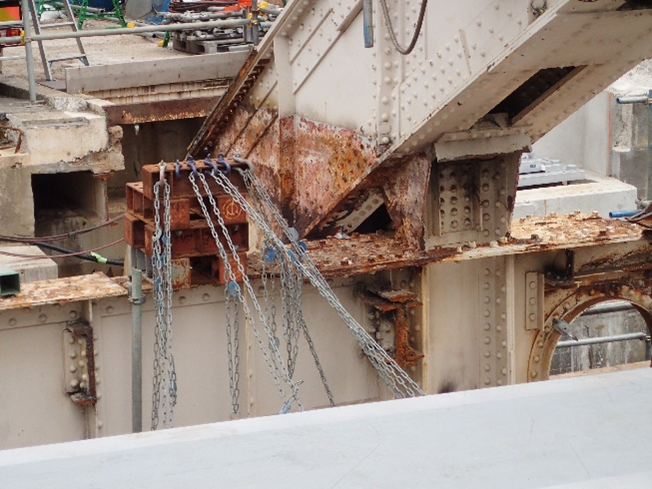
\includegraphics[]{imgs/ch2/rivet-cor.png}
        \caption{Corrosion of rivet}
        \label{fig-corriv}
    \end{subfigure}
    \hfill
    \begin{subfigure}[t]{0.55\linewidth}
        \centering
        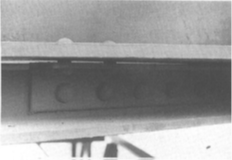
\includegraphics[]{imgs/ch2/rivet-loss.png}
        \caption{Loosing of rivet}
        \label{fig-losriv}
    \end{subfigure}
    \caption{Aging condition of rivet}
\end{figure}

\begin{figure}
    \centering
    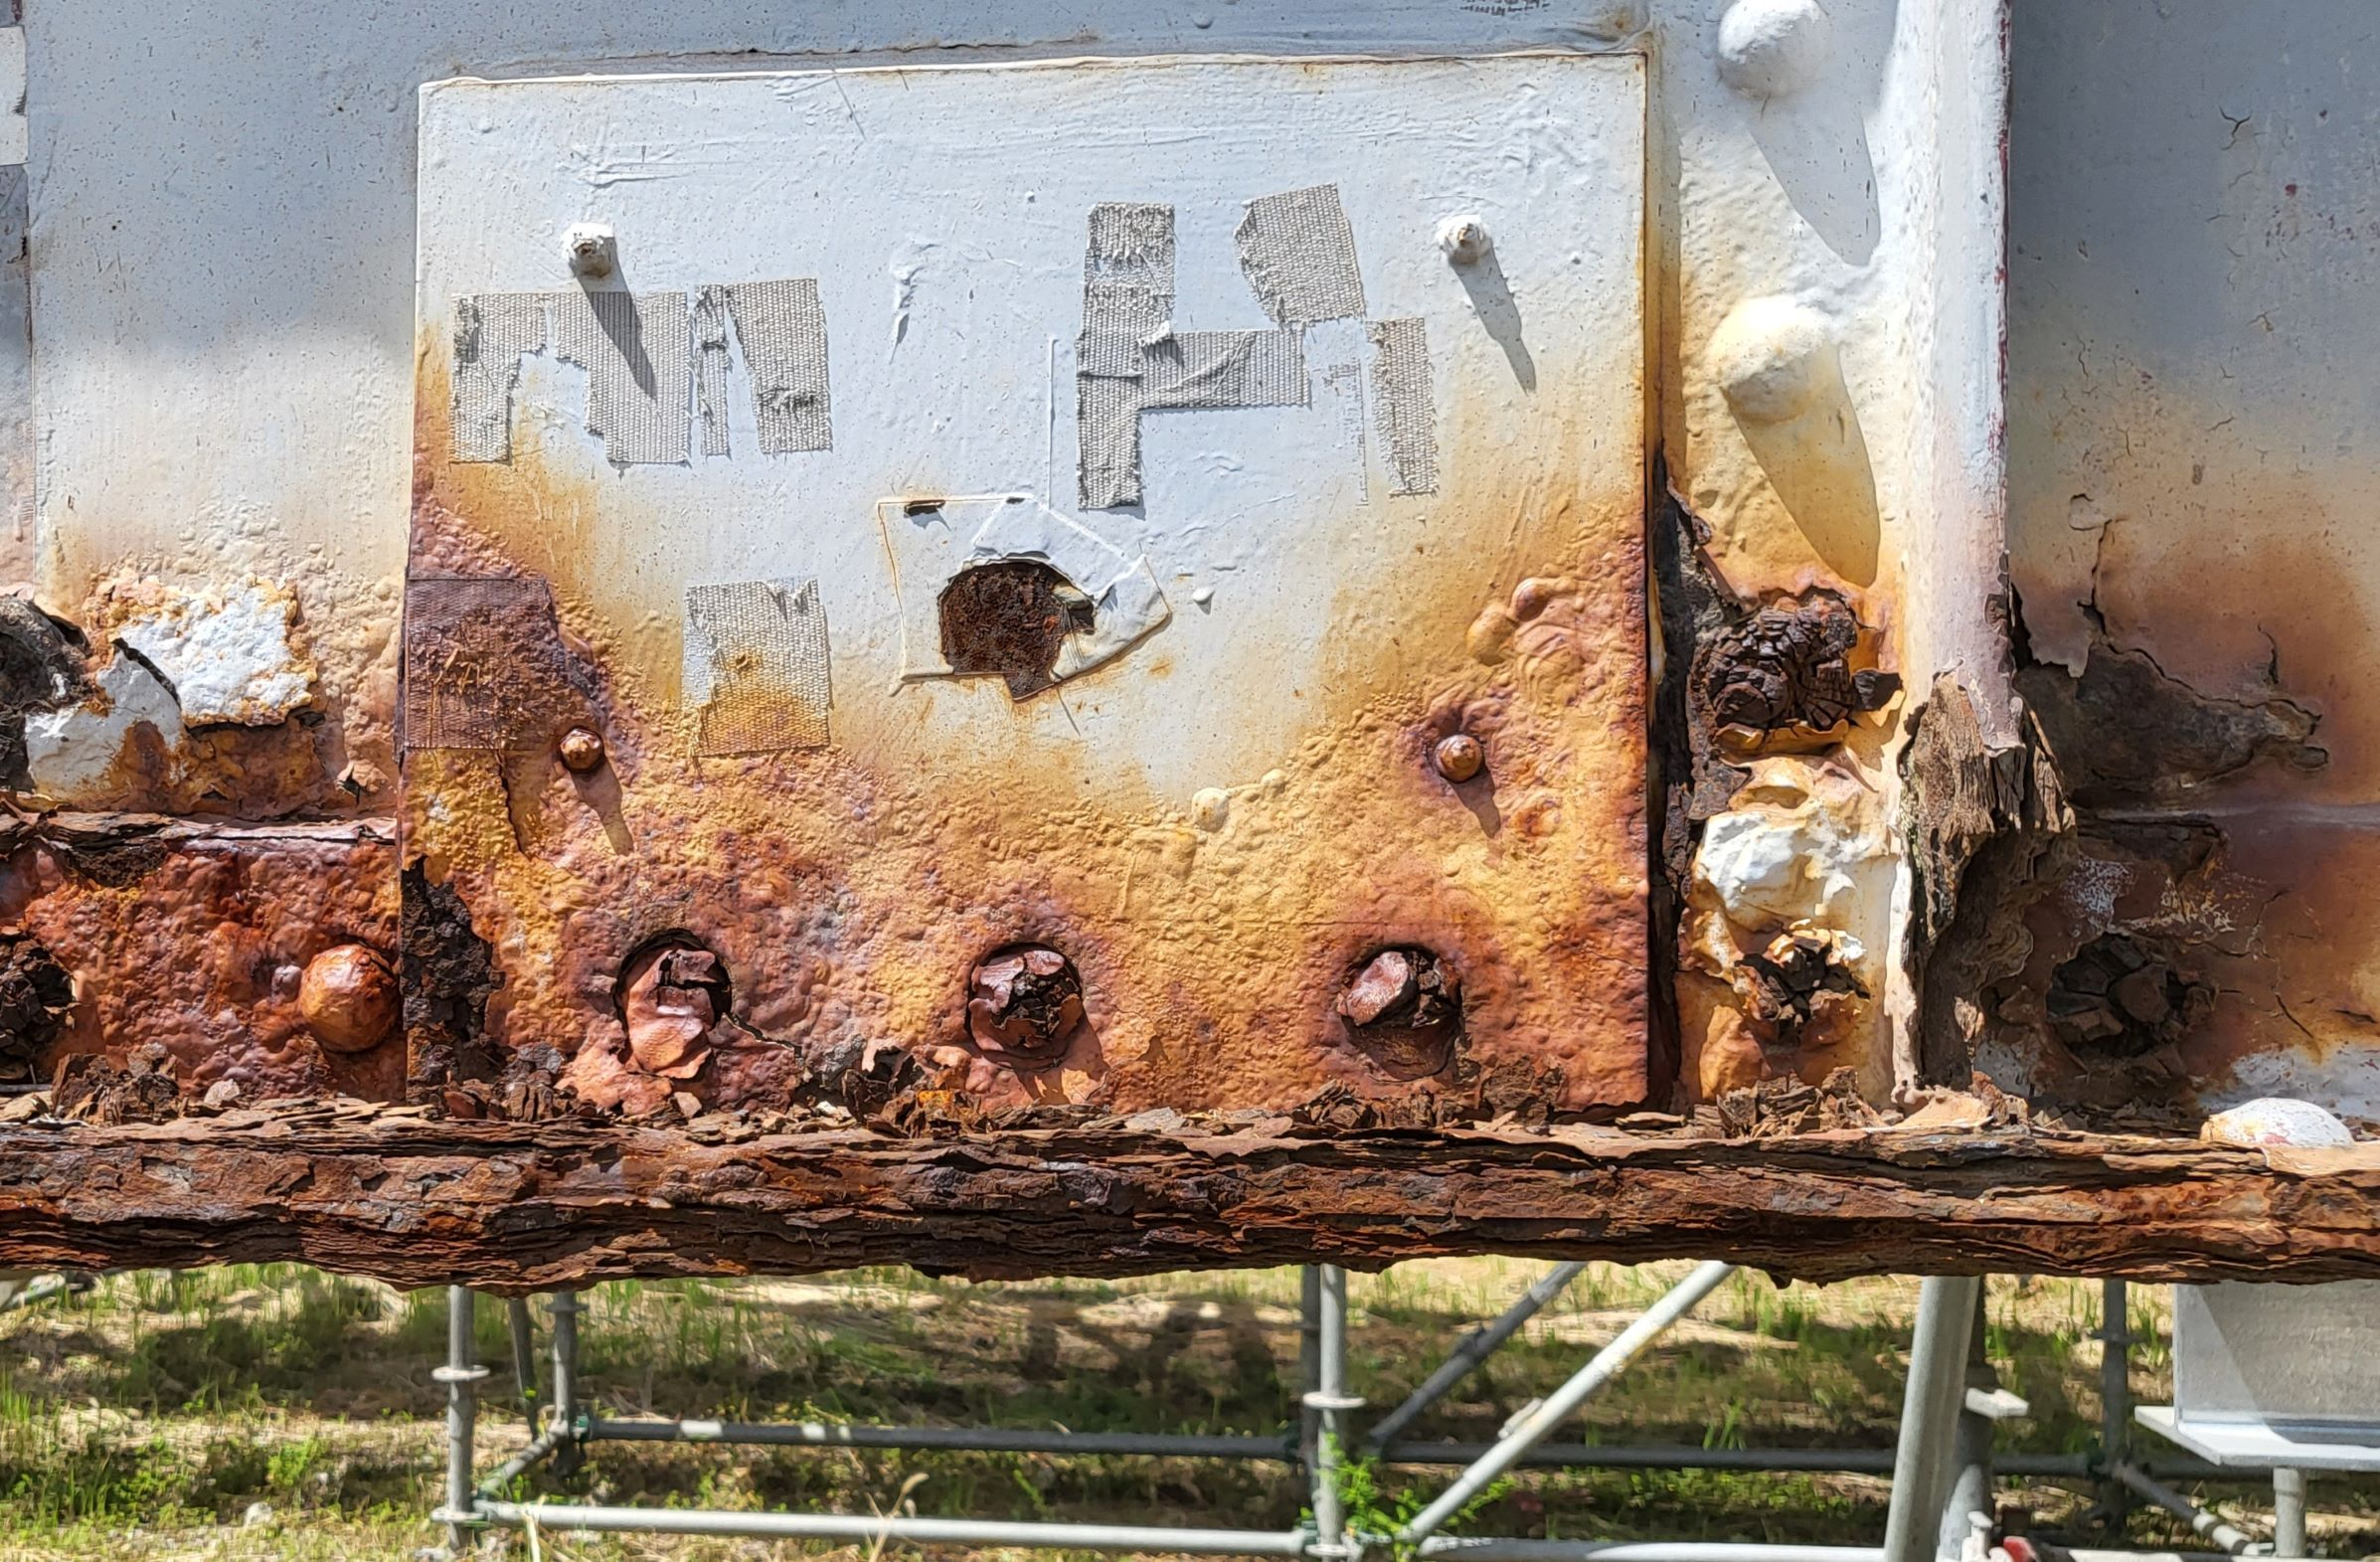
\includegraphics[width=0.8\textwidth]{imgs/ch2/rivet-cor2.jpg}
    \caption{Corrosion of rivet}
    \label{fig-rivet-cor2}
\end{figure}

\subsubsection{Clamping force (Preload) of rivet}

When the heated rivet cools and hardens, the shrinkage of the rivet shaft introduces a significantly higher clamping force. In the past, there have been few studies to assess the clamping force of rivets due to limitations in measurement techniques. In the past, it was believed that the rivet would provide a clamping force equivalent to the yield point of the steel \cite{VanMaarschalkerwaart1982FatigueJoints}. However, subsequent experiments have shown that a clamping force of the yield point of the shaft part can be achieved by incorporating a relatively long rivet shaft ($>100 mm$). In contrast, when a short rivet shaft is present, the mean value of the clamping force introduced is lower, and the dispersion is also higher \cite{Zhou1994FatigueMembers, Baron1953TheJoints}. The deviation of the rivet head is believed to have a significant impact on the clamping force for short rivet axes.

Previous research findings \cite{Zhou1994FatigueMembers} indicate that the clamping force is dependent on the steel grade, particularly for rivets with a diameter of 24.5 mm. Therefore, Åkesson \cite{Akesson2010} refers to the nominal tensile stress caused by the clamping force in the axial section of the rivet as the clamping stress. The clamping stress to yield stress ratio of the rivet material was a crucial parameter in assessing the rivet clamping force. The average ratios were 0.61 and 0.77 for the rivet shaft lengths of 75 mm and 125 mm respectively. K{\"u}hn \cite{Kuhn2008AssessmentLife} have shown that the tightening force of st52 material rivets is lower than that of st37 material rivets.

The above mentioned previous studies mainly conducted tests in laboratory settings utilizing relatively long rivet shafts. Nevertheless, the actual clamping force introduced during riveting real bridges, particularly in-situ, differs to some extent from these experimental findings due to mistakes made during the riveting operation. A previous study8) removed rivets from real bridge girders and flanges to measure the residual rivet clamping force. Akesson \cite{Akesson2010} and Baron \& Larsson \cite{Baron1953TheJoints} reported comparable outcomes. Both sets of experimental data indicated that the length of the rivet shaft had a significant impact on the clamping force. Fig.\ref{fig-preload-rivet} showed that a relatively long rivet shaft increased the average clamping force while decreasing its variance. Moreover, Leonetti \cite{Leonetti2020RivetBridges} also found that the number of plates also had an influence on the clamping force of the rivet. It has been reported that the misalignment of the plates' holes was caused by construction errors.

\begin{figure}
    \centering
    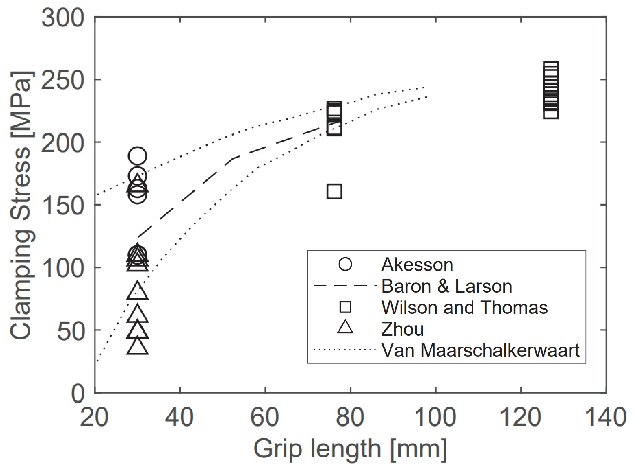
\includegraphics[width=0.8\textwidth]{imgs/ch2/preload-rivet.pdf}
    \caption{The variability of the clamping stress as a function of the grip length for carbon steels. figure cite from \cite{Leonetti2020RivetBridges}, experimental data from Åkesson \cite{Akesson2010},Wilson and Thomas \cite{Wilson1938FatigueJoints}, and Zhou \cite{Zhou1994FatigueMembers}. Also the average trend from Baron \& Larson \cite{Baron1953TheJoints}, and upper and lower bounds from van Maarschalkerwaart \cite{VanMaarschalkerwaart1982FatigueJoints} are reported.}
    \label{fig-preload-rivet}
\end{figure}


\subsubsection{Mechanical behavior of riveted joint}

There are three types of resistance acting on a riveted joint: friction, bearing and shear. There are two types of force transfer using a single rivet: two plates stacked and connected (single shear) and two plates sandwiched and connected (double shear). Although an increase in the number of plates results in a multi-sided shear, the above two types are the basic structures of riveted joints when classified in terms of the action of forces. The forces transmitted by the rivet only consider forces perpendicular to the rivet axis and do not take into account the action of axial tensile forces on the rivet head or its design. When two plates are riveted together, frictional forces act to limit the movement of the plates, which also acts as the strength of the joint, but this is not considered in the design. As shown in Figure 1-7, the stress distribution in the joint, including the rivet and the plate, is extremely complex, but for practical purposes it can be divided into the following three types for ease of handling. The load transfer mechanisms of high strength bolted and riveted joints are shown in Figure 1-8. High-strength bolted joints transmit loads by frictional forces on the joint surfaces by applying high axial forces. In contrast, riveted joints do not take friction into account in their design because it is difficult to control the clamping force and the load is transmitted by the bearing resistance and shear resistance of the rivet shaft. Riveted joints are also very rigid as the rivet head deforms to clamp the plate and cannot be semi-permanently removed once tightened.


\section{Friction type bolted joint}

\section{Bearing type bolted joint}


\begin{equation}
F_{\mathrm{v}, \mathrm{Rd}}=\frac{\alpha_{\mathrm{v}} f_{\mathrm{ub}} A_{\mathrm{s}}}{\gamma_{\mathrm{M} 2}}
\end{equation}



\section{Installation methods for Interference-fit bolt}

\section{Hybrid Connection}

\subsection{Rivet-HSB}

\subsection{HSB-IFB}

\subsection{HSB-Weld}
\label{sec-hsbweld}

Adding Welds to Mechanically Fastened Joints Welded connections are rigid. Welded connections are stiff. Unlike snug-tightened bolted joints that may slip as they are loaded, welds are not expected to stretch and distribute the applied load to any great extent. In most cases, welds and bearing-type mechanical fasteners won't deform equally.

When welds and mechanical fasteners are used together, load is transferred through the stiffer part; therefore, the weld can carry almost all the load, sharing little with the bolts. That's why caution needs to be taken when welds, bolts, and rivets are combined.Code Provisions. The issue of mixing mechanical fasteners and welds is addressed in the AWS D1. 1:2000 Structural Welding Code—Steel. Provision 2.6.3 states that for rivets or bolts used in bearing-type connections (that is, when the bolt or rivet acts as a pin), the mechanical fasteners shouldn't be considered as sharing the load in combination with welds. If welds are used, they should be provided to carry the entire load in the connection. However, connections that are welded to one member and riveted or bolted to another are permitted.

https://www.thefabricator.com/thefabricator/article/arcwelding/mixing-welds--bolts
https://pressbooks.bccampus.ca/powr4406/chapter/bolted-and-welded-joints/

\section{Regulations and standards}

\subsection{Riveted joint}

Shear resistance, per shear plane, Eurocode:
\begin{equation}
F_{\mathrm{v}, \mathrm{Rd}}=\frac{0,6 f_{\mathrm{ur}} A_0}{\gamma_{\mathrm{M} 2}}
\end{equation}